\chapter{Fejlesztői dokumentáció} % Developer guide
\label{ch:impl}

\section{A NES felépítése}

\begin{figure}[H]
	\centering
	\includegraphics[scale=0.22]{mobo.jpg}
	\caption{A NES alaplapja}
\end{figure}

A NES emulációjához a következő komponenseket kell megismernünk és megvalósítanunk:

\begin{compactdesc}
	\item[Ricoh RP2A03:] A hangchipet és központi feldolgozóegységet tartalmazó integrált áramkör. Utóbbi nem más, mint az Apple II-ben és Commodore 64-ben használt 8-bites MOS Technology 6502.
	\item[Ricoh RP2C02:] A képfeldolgozó egység, rövid nevén PPU (Picture Processing Unit).
	\item[NROM és UNROM:] 
	A két megvalósított Mapper áramkör.
	A feladatuk megegyezik a mai számítógépekben is megtalálható MMU-kéval, azaz a virtuális memóriacímeket a kazettán található fizikai címekre alakítják át.
\end{compactdesc}

\section{Órajel-frekvenciák}
A párhuzamosan működő komponenseket az órajelek hangolják össze. Az órajel-frekvencia határozza meg, hogy egy másodperc alatt hány atomi műveletet végez el egy komponens.
Minden komponens rendelkezik egy saját órajelfrekvenciával, amit egy központi órajelből származtatnak.

\begin{itemize}
	\item Központi órajel-frekvencia: $ f = \frac{236.25\;MHz}{11} \sim 21.477272\; MHz $
	\item CPU órajel-frekvencia: $ \frac{f}{12} \sim 1.789773 \; MHz  $
	\item PPU órajel-frekvencia: $ \frac{f}{4}  \sim 5.369318 \; MHz $
\end{itemize}

\section{A központi feldolgózóegységhez kapcsolódó fogalmak}

\begin{note}
A hexadecimális értékeket \textbf{\$} prefix-el jelölöm.
\end{note}

\subsection{Opkód} 
Egy opkód ennél a processzornál csupán egyetlen bájt, amiből az utasításdekódoló egyértelműen meg tudja határozni a végrehajtandó utasítást és annak címzési módját.
Ezt a hozzárendelést az opkódmátrix írja le.
Az emulációhoz tárolni kell az opkódmátrixban, 
hogy a végrehajtandó művelet hány központi órajel alatt fejeződik be.
Azok az opkódok csillaggal vannak jelölve, amiknek futási ideje csak végrehajtás során dönthető el, az aktuális argumentumok alapján. 

\begin{figure}[H]
	\centering
	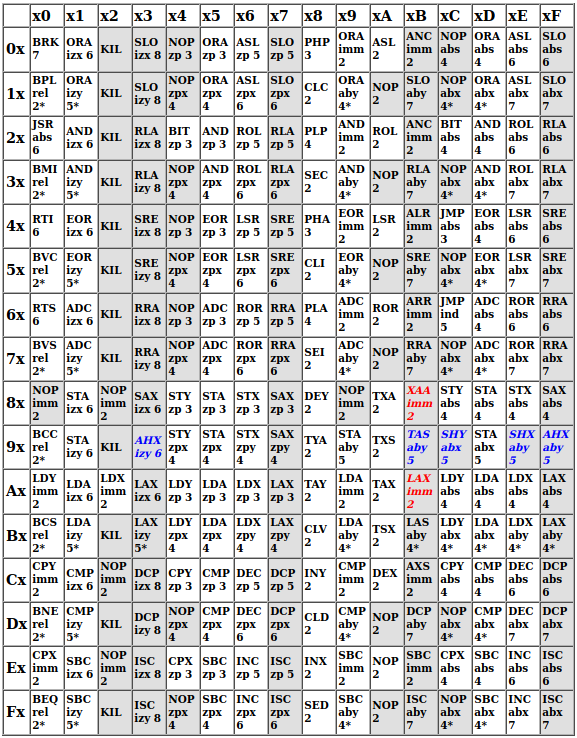
\includegraphics[scale=0.65]{opcodes.png}
	\caption{A 6502 opkódmátrixa}
	\label{fig:opcodes}
\end{figure}

Ha egy opkódhoz meg szeretnénk találni a hozzá tartozó információkat, akkor szükségünk lesz az opkód hexadecimális alakjára, ami legfeljebb két számjegyű lehet. A nagyobb helyiértékű számjegy a keresett cella sorát, a kisebbik pedig az oszlopát írja le. Példaként a \ref{fig:opcodes} ábrán láthatjuk, hogy a \textbf{\$30} opkódhoz a BMI utasítás tartozik relatív címzéssel.
A szürkével jelölt opkódokhoz hivatalosan nincs utasítás rendelve. 
Ezeket a nem dokumentált, "illegális" opkódokat a processzor későbbi 
verzióinak hagyták fent. A tervezők nem tiltották meg azonban ezeknek a használatát, 
egyszerűen csak nem definiálták a viselkedésüket. Ennek ellenére több olyan illegális opkód is belekerült a dizájnba, ami később hasznosnak bizonyult. A fejlesztők próbálkozások útján
felfedezték, hogy melyek azok az opkódok, amiknek a viselkedése determinisztikus és néhány speciális feladat esetén érdemes őket használni.
Ritka ugyan, de van olyan játék, ami ezeket az opkódokat is használja, így ajánlott ezeket is emulálni.

\subsection{Regiszterek}
A regiszter a processzor leggyorsabban elérhető memóriája.
A gyártási költségek alacsonyan tartása végett csak 6 regiszter került a processzorba.

\begin{compactdesc}
	\item[A:] Akkumulátor, az aritmetikai műveletek eredményei ebbe kerülnek.
	\item[X és Y:] 
	Index regiszterek, indirekt címzésnél használjuk őket.
	Ciklusok esetén a ciklusváltozót érdemes ezekben tárolnunk.
	\item[S:] 
	Verem mutató. A verem tetejének a kezdőcímtől vett eltolását tárolja.
	\item[P:]
	Státusz regiszter, ami 7 darab flag bitet tárol.
	\item[PC:]
	Programszámláló. A következő opkód memóriacímét tárolja.
	A többi regiszterrel ellentétben ez nem 8, hanem 16 bites.
	Ebből következik, hogy a processzor címtartományának mérete 64 KiB.
\end{compactdesc}


\subsection{Memórialap}
Az $i$. lap a $ [i \cdot \$FF, (i+1) \cdot \$FF] $ címtartományon elhelyezkedő, 256 bájtos egybefüggő memóriarész.

\subsection{Hívási verem}
Az egymásba ágyazott eljárásokat a processzor hardveresen támogatja, amihez egy vermet használ.
A verem az 1. lapon található, és a kisebb címek felé nő.
Eljárás hívásakor a verem tetejére kerül az aktuális programszámláló értéke, 
visszatéréskor pedig a veremről levett címre állítjuk be a programszámláló értékét.

\subsection{Megszakítás}
A komponensek kommunikációjának egyik módja a hardveres megszakítás.
A 6502 chip egy darab maszkolható \emph{(IRQ)} és egy nem maszkolható \emph{(NMI)} megszakítási lábbal rendelkezik.
A megszakítási vektorral a program megszabhatja, hogy adott megszakítás esetén a vezérlés melyik szubrutinhoz ugorjon. Például ha van egy szubrutin, amit NMI esetén futtatni szeretnénk, akkor a \textbf{\$FFFA} és a \textbf{\$FFFB} címekre be kell írni a szubrutin címét, a kevésbé szignifikáns bájttal kezdve.
A program dönthet úgy, hogy a maszkolható megszakítást figyelmen kívül hagyja, ehhez a megfelelő flag-et be kell állítania a státusz regiszterben. A nem maszkolható megszakítást esetén erre nincsen lehetőség, a végrehajtás mindenképpen a kezelő szubrutinhoz ugrik.
A nem maszkolható lábhoz a képfeldolgozó, a maszkolhatóhoz a hangchip van kötve.

\subsection{Opkód argumentumok fajtái}

\begin{figure}[H]
	\centering
	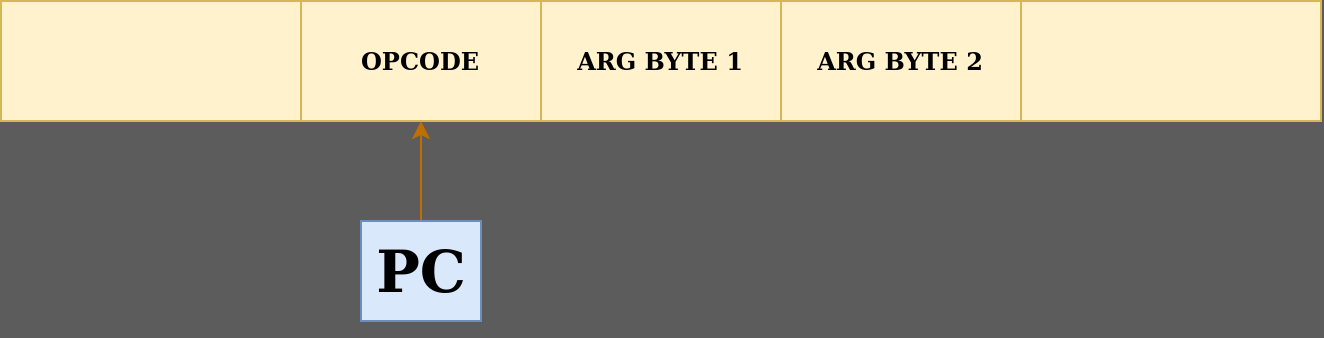
\includegraphics[scale=0.25]{opcode.png}
	\caption{Opkód argumentumainak helye}
\end{figure}

\begin{compactitem}
	\item Abszolút memóriacím (16 bit)
	\item Eltolást leíró bájt
	\item Közvetlen operandusként szolgáló bájt
\end{compactitem}

\subsection{Címzési módok}

Egy opkód után azoknál a címzési módoknál áll argumentum, amiknél a művelet elvégzéséhez 
szükséges operandus nem regiszterben, hanem a memóriában van. A címzési módok azt határozzák meg, hogy az argumentumból hogyan kell kiszámolni az operandus effektív 16 bites memóriacímét. A címzési mód mögött álló zárójelben az opkódmátrixbeli név (amennyiben van) és az argumentumok száma található.  


\begin{description}
	\item[Akkumulátor mód (0):] nincs argumentum, az utasítás az \textbf{A} regiszter értékét módosítja.
	\item[Azonnali mód (imm, 1):] az utasítás operandusa maga az argumentum. Jele: \#
	\newline
	Példa: az LDA \#\$0 utasítás nullára állítja az \textbf{A} regisztert.
	\item[Abszolút mód (abs, 2):] a paraméter az operandus effektív címe.
	\item[0. lap mód (zp, 1):] A CPU kevés regiszterét azzal ellensúlyozták, hogy ennek a speciális módnak köszönhetően a nulladik lapot hatékonyabban lehet címezni, mint a többit. 
	Mivel a 0. lap mérete 256 bájt, ezért teljes cím helyett elég egyetlen bájt a címzéséhez.
	A kisebb paraméter gyorsabban beolvasható és egyúttal a kódméretet is csökkenti.
	\item[Indexelt 0. lap mód (zpx, zpy, 1):]
	Hasonlóan most is csak a 0. lapot tudjuk címezni, de az argumentumhoz hozzáadjuk valamelyik index regiszter értékét.
	Az operandus címének kiszámítása: $ (arg1 + index) \mod 256 $
	\item[Indexelt abszolút mód (abx, aby, 2):] Az argumentum egy teljes memóriacím, amihez hozzáadjuk a megadott index regiszter értékét. 
	\item[Adott mód (0):] nincs szükség argumentumra, mert az utasítás regiszterekkel dolgozik.
	\item[Relatív mód (rel, 1):] Elágazásoknál ha a feltétel teljesül, akkor az argumentummal el kell tolni a programszámlálót.
	\item[Indirekt mód (ind, 2):] 
	Erre a címzési módra a JMP utasításnál van szükség.
	A két argumentum bájt együtt egy teljes memóriacímet alkot, legyen ez \emph{m}.
	Az operandus címét innen kell kiolvasnunk, vagyis a következőképpen kapjuk meg: $ (read(m+1) << 8) \;\; | \;\; read(m) $ 
	\item[Indexelt indirekt mód (izx, 1):]
	Az X regisztert összeadjuk az argumentummal, így egy 0. lapon található címet kapunk.
	Ezen címen az alsó, a következőn pedig a felső 8 bitje található az operandus effektív memóriacímének.
	\begin{figure}[H]
		\centering
		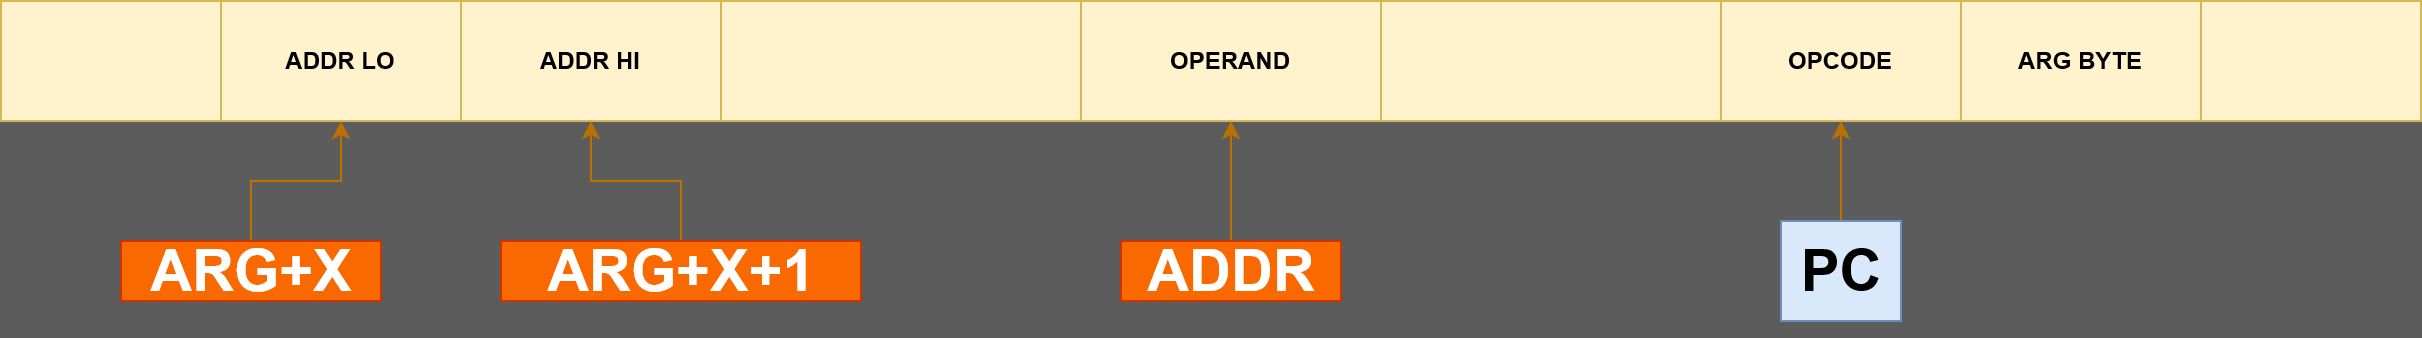
\includegraphics[width=1.1\textwidth,height=70px]{indexed_indirect.png}
		\caption{Indexelt indirekt címzés}
	\end{figure}
	\item[Indirekt indexelt mód (izy, 1):]
	Az argumentum egy 0. lapon található címre mutat, amit ha összeadunk az Y regiszter értékével, akkor megkapjuk az operandus effektív címét. 
	
	
	
\end{description}

\subsection{Memóriatérkép}

A memóriatérkép leírja a címtér felosztását a komponensek között.
A memóriatérképből meg tudjuk állapítani, hogy egy adott címen található bájt kiolvasásához vagy írásához melyik komponens hardveres logikáját kell alkalmazni.

\begin{table}[H]
	\centering
	\begin{tabular}{ | l | l | }
		\hline
		Tartomány & Eszköz \\
		\hline			
		$ \$0000 - \$07FF $ & CPU RAM \\
		$ \$0800 - \$1FFF $ & A CPU RAM tükrözése \\
		$ \$2000 - \$2007 $ & PPU regiszterek \\
		$ \$2008 - \$3FFF $ & PPU regiszterek tükrözése \\
		$ \$4000 - \$4017 $ & APU és IO regiszterek \\
		$ \$4018 - \$401F $ & APU és IO regiszterek tükrözése \\
		$ \$4020 - \$FFFF $ & Kazetta \\
		\hline
	\end{tabular}
\end{table}

\subsection{Memóriatükrözés}
Memóriatükrözésről beszélünk, amikor fizikailag ugyanazt a memóriaterületet több memóriacímről is el tudjuk érni. Ha egy címtartomány $x$ bájtonként tükrözve van, akkor minden olyan $a$ és $b$ memóriacím ugyanarra a bájtra mutat, ami a tartományba vagy a tükrözésébe esik és $a \equiv b\ (\textrm{mod}\ x)$.  A CPU RAM 2 KiB-onként tükrözve van, amiből következik, hogy a \textbf{\$0001}, \textbf{\$0801} \textbf{\$1001}, \textbf{\$1801} címek ugyanarra a bájtra mutatnak.

\subsection{Státusz flagek}

\begin{compactenum}
	\setcounter{enumi}{-1}
	\item bit: C = Carry
	\item bit: Z = Zero
	\item bit: I = IRQ Disable
	\item bit: D = Decimal mode
	\item bit: B = BRK Command
	\setcounter{enumi}{5}
	\item bit: V = Overflow
	\item bit: N = Negative
\end{compactenum}

\subsection{Utasításkészlet}

\begin{compactdesc}
	\item Aritmetikai és logikai egység (ALU)
	\begin{compactdesc}
		\item[ADC:] Összeadás
		\item[SBC:] Kivonás
		\item[AND:] Logikai ÉS művelet
		\item[ASL:] Bájt balra elcsúsztatása
		\item[LSR:] Bájt jobbra elcsúsztatása
		\item[ORA:] Logikai VAGY
		\item[EOR:] Kizárásos VAGY
		\item[INC, INX, INY:] növelés eggyel
		\item[DEC, DEX, DEY:] csökkentés eggyel
		\item[ROL, ROR:] bájt forgatása
	\end{compactdesc}
	\item 
	Összehasonlítás \newline \textbf{CMP, CPX, CPY}
	\item Veremműveletek
	\begin{compactdesc}
		\item[PHA:] Az akkumulátor regiszter értékének felrakása a veremre 
		\item[PHP:] A státusz regiszter értékének felrakása a veremre
		\item[PHA:] Az akkumulátor regiszter új értékének levétele a veremről
		\item[PHP:] A státusz regiszter új értékének levétele a veremről
	\end{compactdesc}
	\item Vezérlés
	\begin{compactdesc}
		\item[JMP:] Vezérlés áthelyezése egy megadott memóriacímhez, avagy a programszámláló átállítása erre a címre.
		\item[JSR:] Szubrutin hívás (visszatérési cím elmentése + \textbf{JMP})
		\item[RTS:] Visszatérés szubrutinból (visszatérési cím kiolvasása + \textbf{JMP})
		\item[BRK:] Szoftveresen generált megszakítás
		\item[RTI:] Visszatérés megszakításkezelőből
	\end{compactdesc}
	\item Flag manipuláció \newline \textbf{CLC, CLD, CLI, CLV, SED, SEC, SEI}
	\newline
	(C = Clear, S = Set)
	\item Elágazások: vezérlés áthelyezése valamelyik státusz regiszterben található flag értéke szerint 
	\newline \textbf{BCC(C=0), BCS(C=1), BNE(Z=0), BEQ(Z=1), BPL(N=0), BMI(N=1),  BVC(V=0), BVS(V=1)}
	\item Bájtok mozgatása regiszterek és a memória között
	\newline
	\textbf{LDA, LDX, LDY, STA, STX, STY} 
	\newline
	(L = Load, S = Store)
	\item Bájtok mozgatása regiszterek között
	\newline
	\textbf{TAX, TAY, TSX, TXA, TXS, TYA}
	\newline
	A név második betűje a forrásregisztert, a harmadik a célregisztert jelöli.
\end{compactdesc}

\section{Kazetták}

\subsection{A kazetta memóriája}

\begin{itemize}
	\item PRG ROM: A program utasításainak tárolására szolgál. 
	\begin{compactdesc}
		\item[NROM:]  16 KiB vagy 32 KiB
		\item[UNROM:] 64 KiB vagy 128 KiB
	\end{compactdesc}
	\item CHR: A játékok képi világának építőelemeit, a $8 \cdot 8$ pixeles sprite-okat tárolja.
	\begin{compactdesc}
		\item[NROM:]  8 KiB ROM
		\item[UNROM:] 8 KiB RAM
	\end{compactdesc}
\end{itemize}

\subsection{Az iNES fájl formátum}


